\documentclass[a4paper,twoside]{article}
\usepackage[T1]{fontenc}
\usepackage[bahasa]{babel}
\usepackage{graphicx}
\usepackage{graphics}
\usepackage{float}
\usepackage[cm]{fullpage}
\pagestyle{myheadings}
\usepackage{etoolbox}
\usepackage{setspace} 
\usepackage{lipsum} 
\setlength{\headsep}{30pt}
\usepackage[inner=2cm,outer=2.5cm,top=2.5cm,bottom=2cm]{geometry} %margin
% \pagestyle{empty}
\usepackage{hyperref}

\hypersetup{unicode=true,colorlinks=true,linkcolor=blue,citecolor=green,filecolor=magenta, urlcolor=cyan}

\graphicspath{{Gambar/}}

\makeatletter
\renewcommand{\@maketitle} {\begin{center} {\LARGE \textbf{ \textsc{\@title}} \par} \bigskip {\large \textbf{\textsc{\@author}} }\end{center} }
\renewcommand{\thispagestyle}[1]{}
\markright{\textbf{\textsc{Laporan Perkembangan Pengerjaan Skripsi\textemdash Sem. Ganjil 2020/2021}}}

\onehalfspacing
 
\begin{document}

\title{\@judultopik}
\author{\nama \textendash \@npm} 

%ISILAH DATA BERIKUT INI:
\newcommand{\nama}{Stephen Hadi}
\newcommand{\@npm}{2017730016}
\newcommand{\tanggal}{12/01/2021} %Tanggal pembuatan dokumen
\newcommand{\@judultopik}{Analisa dan Implementasi Perbaikan Perangkat Lunak BlueTape} % Judul/topik anda
\newcommand{\kodetopik}{PAN4901}
\newcommand{\jumpemb}{1} % Jumlah pembimbing, 1 atau 2
\newcommand{\pembA}{Pascal Alfadian}
\newcommand{\pembB}{-}
\newcommand{\semesterPertama}{49 - Ganjil 20/21} % semester pertama kali topik diambil, angka 1 dimulai dari sem Ganjil 96/97
\newcommand{\lamaSkripsi}{1} % Jumlah semester untuk mengerjakan skripsi s.d. dokumen ini dibuat
\newcommand{\kulPertama}{Skripsi 1} % Kuliah dimana topik ini diambil pertama kali
\newcommand{\tipePR}{B} % tipe progress report :
% A : dokumen pendukung untuk pengambilan ke-2 di Skripsi 1
% B : dokumen untuk reviewer pada presentasi dan review Skripsi 1
% C : dokumen pendukung untuk pengambilan ke-2 di Skripsi 2

% Dokumen hasil template ini harus dicetak bolak-balik !!!!

\maketitle

\pagenumbering{arabic}

\section{Data Skripsi} %TIDAK PERLU MENGUBAH BAGIAN INI !!!
Pembimbing utama/tunggal: {\bf \pembA}\\
Pembimbing pendamping: {\bf \pembB}\\
Kode Topik : {\bf \kodetopik}\\
Topik ini sudah dikerjakan selama : {\bf \lamaSkripsi} semester\\
Pengambilan pertama kali topik ini pada : Semester {\bf \semesterPertama} \\
Pengambilan pertama kali topik ini di kuliah : {\bf \kulPertama} \\
Tipe Laporan : {\bf \tipePR} -
\ifdefstring{\tipePR}{A}{
			Dokumen pendukung untuk {\BF pengambilan ke-2 di Skripsi 1} }
		{
		\ifdefstring{\tipePR}{B} {
				Dokumen untuk reviewer pada presentasi dan {\bf review Skripsi 1}}
			{	Dokumen pendukung untuk {\bf pengambilan ke-2 di Skripsi 2}}
		}
		
\section{Latar Belakang}

 Berkembangnya FTIS UNPAR disertai dengan tersedianya semakin banyak matakuliah, dari perkembangan tersebut muncul permasalahan baru di bagian bidang administrasi. Jika dosen ingin meniadakan perkuliahan atau mengganti perkuliahan akan tidak efisien jika melakukan panggilan atau \textit{email} ke pihak tata usaha. Hal tersebut akan memberatkan pihak tata usaha. Mahasiswa yang ingin melakukan pengajuan transkrip akan membuang waktu dan tenaga, karena saat mahasiswa ingin melakukan pengajuan transkrip maka mahasiswa harus datang ke tata usaha melakukan pengajuan dan menunggu beberapa hari untuk mendapatkan hasil transkrip tersebut. Mahasiswa yang tidak memiliki perkuliahan pada hari tersebut harus datang hanya untuk melakukan pengajuan. Hal ini selain membuang waktu juga membuang biaya transportasi.


\textit{Bluetape} adalah aplikasi web yang dibuat oleh dosen dan mahasiswa informatika. Aplikasi ini dibuat menggunakan \textit{Hypertext Preprocessor} atau lebih dikenal dengan \textit{PHP}. \textit{Database management system} atau DBMS yang digunakan adalah \textit{MYSQL}.\textit{ Bluetape} menggunakan \textit{framework Bootstrap} dan \textit{Codeigniter}. \textit{Bluetape} berguna untuk membantu kegiatan administrasi FTIS UNPAR. Aplikasi ini dapat melakukan \textit{transkrip request/manage} dan \textit{request perubahan kuliah/manage}. Sehingga jika dosen ingin meniadakan/mengganti perkuliahan dapat dilakukan dengan mudah tanpa harus membuat email ataupun melakukan panggilan. Mahasiswa dapat melakukan permintaan transkrip nilai tanpa tatap muka sehingga mahasiswa hanya perlu datang ke UNPAR saat ingin mengambil hasil dari transkrip tersebut, selain itu mahasiswa juga dapat melihat jadwal dosen. Dengan adanya sistem otomasi pada kegiatan administrasi tentunya pekerjaan tata usaha menjadi lebih ringan. 


Aplikasi \textit{Bluetape} digunakan oleh mahasiswa FTIS, dosen ,dan tata usaha. Dari pengguna--pengguna tersebut tentu akan ada hal yang disukai dan hal yang tidak disukai. Seperti ada fitur yang bermasalah, ada fitur yang kurang atau hanya saran untuk fitur kedepannya yang akan memudahkan kegiatan administrasi dalam FTIS UNPAR. Dengan adanya masukan--masukan dari pengguna maka aplikasi \textit{Bluetape} dapat ditingkatkan penggunaannya dan memperbaiki kelemahan dari \textit{Bluetape}.

Pada topik skripsi ini akan dilakukan analisis untuk perbaikan dan penambahan fitur untuk aplikasi \textit{Bluetape}, penambahan fitur akan disurvei kepada semua pengguna \textit{Bluetape}. Pengguna yang akan disurvei tidak semua. Hanya perwakilan--perwakilan dari pihak dosen, tata usaha, dan mahasiswa. Selanjutnya akan dianalisa bersama pembimbing untuk menentukan fitur yang akan dirancang dan diimplementasi. Survei tidak terbatas hanya pada fitur tambahan, fitur--fitur yang tidak menghasilkan sesuai kegunaannya akan diperbaiki juga.


Sebelum melakukan perancangan dan implementasi diperlukan untuk \textit{setup} aplikasi \textit{Bluetape} pada komputer sendiri dan ada persyaratan yang harus dipenuhi yaitu mendaftarkan diri ke \textit{google OAuth 2.0} diakrenakan \textit{login} pada \textit{Bluetape} menggunakan akun \textit{gmail} UNPAR. Selanjutnya juga akan dipelajari \textit{framework CodeIgniter dan Bootstrap} yang menjadi dasar dari aplikasi ini.

\section{Rumusan Masalah}

Rumusan masalah yang telah diidentifikasi sebagai berikut:
\begin{enumerate}
	\item Apa sajakah kebutuhan yang diinginkan oleh pengguna bluetape?
	\item Bagaimana menganalisa, merancang, dan mengimplementasi \textit{feedback--feedback} dari pengguna?
	\item Bagaimana melakukan pengujian setelah mengimplementasi \textit{feedback--feedback} dari pengguna?
	
\end{enumerate}

\section{Tujuan}

Tujuan pembuatan dan penulisan skripsi ini adalah sebagai berikut:
\begin{enumerate}
	\item Mendapatkan \textit{feedback--feedback} dari pengguna terkait kebutuhan yang diinginkan.
	\item Menganalisa, merancang, dan mengimplementasi \textit{feedback--feedback} dari pengguna
	\item Melakukan pengujian setelah mengimplementasi semua \textit{feedback} yang memungkinkan untuk diimplementasi
	
\end{enumerate}

\section{Detail Perkembangan Pengerjaan Skripsi}
Detail bagian pekerjaan skripsi sesuai dengan rencan kerja/laporan perkembangan terkahir :

\begin{enumerate}
	\item \textbf{Memahami dan mengerti cara kerja \textit{framework} \textit{Code igniter}, \textit{Bootstrap}, \textit{Phpspreadheet}, dan \textit{Google OAuth 2.0}.}\\
	{\bf Status :} Ada sejak rencana kerja skripsi, kecuali \textit{phpspreadsheet} dan \textit{Google OAuth 2.0}.\\
	{\bf Hasil :} Cara kerja \textit{code igniter}, \textit{bootstrap}, \textit{phpspreadsheet}, dan \textit{Google OAuth 2.0} telah dipelajari, Hasil dari studi secara garis besar:
	\begin{enumerate}
		\item \textbf{Code Igniter} \\
		\textit{CodeIgniter}\footnote{Version 3.1.11 (2019) \textit{CodeIgniter 3}. British Columbia Institute of Technology. 3700 Willingdon Ave} adalah \textit{framework} untuk pembuatan \textit{website} yang menggunakan \textit{PHP}. \textit{CodeIgniter} mempermudah \textit{developer} untuk meminimalisir penggunaan kode untuk mengakses suatu fungsi.
		
		\begin{figure}[H]
			\centering
			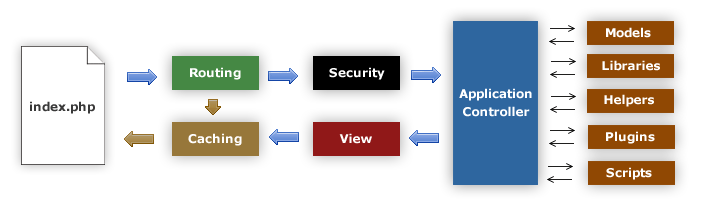
\includegraphics[scale=0.8]{mvc} 
			\caption{Flowchart MVC}
			\label{fig:appflowchart} 
		\end{figure}
				
		 \textit{CodeIgniter} menerapkan arsitektur \textit{MVC} yang dapat dilihat pada gambar \ref{fig:appflowchart}, file \texttt{index.php} berfungsi mengatur routing dan mengarahkan ke \textit{application controller} yang berada di direktori \textit{controller} dan melalui \textit{controller} akan dipanggil \textit{models, libraries, helpers, etc} yang dibutuhkan dengan perintah \texttt{\$this->load}. \textit{MVC} secara umum akan mengolah data pada \textit{models} dan hasil yang sudah siap akan dikirim ke \textit{view} melalui \textit{controller}. Fitur tambahan dari arsitektur \textit{CodeIgniter} adalah saat \textit{router} memeriksa \textit{HTTP request}, jika \textit{cache} tersedia maka akan dikirimkan \textit{cache} tersebut dan jika tidak ada \textit{cache} maka \textit{security} akan memeriksa dan melakukan filter terhadap \textit{HTTP request} seperti pada gambar \ref{fig:appflowchart}. 
		 
		 \textbf{\textit{Controller}} \\
		 \textit{Controller} adalah pusat dari aplikasi, \textit{controller} menangani apa yang harus dilakukan dari \textit{HTTP request}. Dalam \textit{CodeIgniter} untuk menginisiasi \textit{controller} cukup menulis nama kelas diikuti dengan \texttt{extends CI\_Controller}.
		 
		 \textbf{\textit{Model}} \\ \textit{Model} berfungsi sebagai \textit{logic} dari aplikasi. \textit{Model} pada \textit{CodeIgniter} bersifat opsional, tetapi disediakan untuk \textit{developer} yang ingin menggunakan MVC. 
		 
		\textbf{\textit{View}} \\
		\textit{View} tidak pernah dipanggil secara langsung, \textit{view} harus dipanggil melalui \textit{controller}. \textit{View} pada \textit{CodeIgniter} ditaruh pada direktori \textit{view}. Pemanggilan \textit{view} menggunakan \textit{method} \texttt{\$this->load->view(`nama\_view')}.
		
		\textbf{Kelas pada \textit{code igniter}} 
		\begin{itemize}
			\item \textbf{CI\_Loader} \\ 
			\textit{CI\_Loader} adalah kelas yang berfungsi untuk \textit{load elements}. \textit{Elements} dapat berupa \textit{libraries, view files, drivers, helpers, models}. Kelas ini sudah diinisialisasi secara otomatis oleh \textit{code igniter}.
			
			\item \textbf{CI\_Config} \\
			\textit{CI\_Config} adalah kelas yang digunakan untuk mengambil konfigurasi yang dibuat. \textit{Method} yang digunakan: \texttt{item}. \textit{Method} \textit{item} digunakan untuk mengambil variabel \texttt{\$config}.
			
			\item \textbf{CI\_Email} \\
			\textit{CI\_Email} adalah kelas yang berfungsi untuk mempermudah pengiriman \textit{email} yang disediakan oleh \textit{codeigniter}. Kelas ini memiliki \textit{method}: 
			\begin{itemize}
				\item \texttt{from} \\
				\textit{Method} ini digunakan untuk memasang alamat \textit{e-mail} pengirim dan nama pengirim.
				\item \texttt{to} \\
				\textit{Method} ini digunakan untuk menentukan tujuan.
				\item \texttt{subject} \\
				\textit{Method} ini digunakan untuk memasang subjek pesan.
				\item \texttt{message} \\
				\textit{Method} ini digunakan untuk memasang pesan yang ingin dikirim
				\item \texttt{send} \\
				\textit{Method} ini digunakan untuk mengirim pesan.
			\end{itemize}
		\item \textbf{CI\_Input} \\ 
		\textit{CI\_Input} adalah kelas yang digunakan untuk menyaring dan membersihkan data masukan untuk meningkatkan keamanan. \textit{Method} yang digunakan:
		\begin{itemize}
			\item \texttt{post} \\
			\textit{Method} ini berfungsi membaca masukan dengan tipe \textit{post}.
			\item \texttt{server} \\
			\textit{Method} ini berguna untuk mengambil \textit{server data} seperti \texttt{\$\_SERVER}.
		\end{itemize}
		\item \textbf{CI\_Session} \\
		\textit{Session} digunakan untuk mengurus  \textit{user's state} dan melihat aktivitas \textit{user} saat menelusuri situs. Kelas ini sama seperti \texttt{\$\_SESSION} \textit{superglobal}. \textit{Method} yang digunakan:
		\begin{itemize}
			\item \texttt{set\_flashdata} \\
			\textit{Method} ini berguna untuk menyimpan data ke \texttt{\$\_SESSION} \textit{superglobal} dan menandai sebagai \textit{flashdata}. \textit{Flashdata} adalah \textit{session data} yang hanya tersedia untuk permintaan berikutnya dan setelah itu akan dibuang.
			
			\item \texttt{flashdata} \\
			 \textit{Method} ini mengambil nilai dari spesifik \texttt{\$\_SESSION} yang telah ditandai sebagai \textit{flashdata}.
			 
			\item \texttt{set\_userdata} \\
			\textit{Method} ini berguna untuk menyimpan data ke \texttt{\$\_SESSION} \textit{superglobal}.
			
			\item \texttt{userdata} \\
			\textit{Method} ini berguna untuk mengambil \textit{value} untuk \texttt{\$\_SESSION} \textit{item} atau \textit{array} semua data user
			
			\item \texttt{unset\_userdata} \\
			\textit{Method} ini berfungsi untuk membuang data dari \texttt{\$\_SESSION} \textit{superglobal} dengan \textit{key} masukan.
		\end{itemize}	
		\end{itemize}
	
	\item \textbf{Phpspreadsheet} \\
	PhpSpreadsheet adalah \textit{library} yang ditulis dengan bahasa PHP berguna untuk membaca dan menulis file dengan jenis spreadsheet seperti Excel dan LibreOffice Calc\footnote{Version 1.14.1 (2019) \textit{PhpSpreadsheet}. PHPOffice. The Internet.}. Kelas pada \textit{phpspreadsheet}:
	\begin{itemize}		 
		\item \textbf{Spreadsheet} \\ 
		\textit{Constructor} kelas \textit{Spreadsheet} tidak menerima parameter apapun, dan \textit{return value} adalah \textit{mixed}. \textit{Method} yang digunakan pada kelas \texttt{Spreadsheet}:
		\begin{itemize}
			\item \texttt{createSheet} \\
			\textit{Method} ini berfungsi untuk membuat \textit{sheet}.
			\item \texttt{setActiveSheetIndex} \\
			Memilih \textit{sheet} yang ingin dijadikan \textit{active} berdasarkan \textit{index}.
			\item \texttt{getActiveSheet} \\
			Mengembalikan kelas \textit{Worksheet} yang telah dibuat menjadi \textit{sheet} aktif pada \texttt{setActiveSheetIndex}.
		\end{itemize}
	
		\item \textbf{Worksheet} \\
		Kelas \textit{Worksheet} adalah kelas yang mengatur nilai dari \textit{cell}, \textit{cell style}, judul \textit{sheet} dll. \textit{Method} yang digunakan pada kelas \texttt{Worksheet}:
		\begin{itemize}
			\item \texttt{getStyle} \\
			Mengembalikan kelas \texttt{Style}.
			\item \texttt{setCellValue} \\
			mengubah suatu nilai pada \textit{cell} tertentu.
			\item \texttt{mergeCells} \\
			Melakukan \textit{merge} pada \textit{cell}.
			\item \texttt{setTitle} \\
			Berfungsi untuk memberi judul pada \textit{sheet}.
			\item \texttt{getRowDimension} \\
			Mengambil dimensi baris pada baris tertentu.
			\item \texttt{getColumnDimension}\\ 	
			Mengambil dimensi kolom pada kolom tertentu.
		\end{itemize}
	
	\item \textbf{Style} \\
	Kelas \textit{Style} adalah kelas yang mengatur \textit{style} dari suatu \textit{cell} seperti \textit{alignment}, \textit{fill},\textit{font} dll. \textit{Method} yang tersedia pada kelas \texttt{Style}:
	\begin{itemize}
		\item \texttt{getFill} \\
		Mengembalikan kelas \textit{Fill}. untuk mengubah \textit{fill} pada suatu \textit{cell} dapat memanggil \texttt{set\-Fill\-Type()} pada kelas \textit{Fill}.
		\item \texttt{getAlignment} \\
		Mengembalikan kelas \textit{Alignment}, untuk mengubah \textit{alignment} pada suatu \textit{cell} dapat memanggil \texttt{setHorizontal()} atau \texttt{setVertical()} pada kelas \textit{Alignment}.
		\item \texttt{getFont} \\
		 Mengembalikan kelas \textit{Font}, untuk mengubah penebalan kata dapat menggunakan \texttt{setBold()} dengan masukan \textit{boolean}.
	\end{itemize}

	\item \textbf{Xls} \\
	Kelas \texttt{Xls} memiliki 2 tipe yaitu \textit{writer} dan \textit{reader}. Pada penelitian kali ini tipe \textit{Xls} yang digunakan hanya tipe \textit{writer}. \textit{Method} yang digunakan dari kelas \texttt{Xls}: \texttt{save}. \textit{Method} ini berfungsi untuk membuat file \textit{spreadsheet} tersimpan dalam format \textit{xls}.
	\end{itemize}

	\item \textbf{Bootstrap} \\
	\textit{Bootstrap} adalah \textit{framework} paling terkenal untuk membuat \textit{site} yang \textit{mobile-first} dan \textit{res\-pon\-sive}\footnote{Version 4.5 (2020) Bootstrap. Bootstrap. San Francisco, United States.}. Komponen-komponen \textit{bootstrap}:
	\begin{itemize}
		\item \textit{Container} \\
		Kelas \texttt{container} adalah kelas yang dibutuhkan jika ingin menggunakan \textit{bootstrap} grid. Kelas \texttt{container} adalah kelas \textit{responsive} dan \textit{fixed-width}.
		
		\item \textit{Grid} \\
		\textit{Grid} pada \textit{bootstrap} digunakan untuk mengatur \textit{layout} dan \textit{alignment}. \textit{Row} adalah kelas \textit{wrapper} untuk kolom. Kelas \textit{col} akan secara otomatis membagi lebar horizontal dari layout menjadi sama besar.
		
		\item \textit{Table} \\
		Kelas \texttt{table} adalah kelas yang membantu pembuatan \textit{table}. Dengan komponen pendukung yang dapat membuat \textit{table} memiliki \textit{border} ataupun \textit{table} dengan \textit{style striped}.
		
		\item \textit{Pagination} \\
		\textit{Pagination} dibuat menggunakan \texttt{HTML list} yang berada didalam \texttt{<nav>} untuk mengidentifikasikan \textit{pagination} sebagai bagian navigasi kepada pengguna. \textit{Pagination} juga menyediakan komponen pendukung seperti menandai \textit{pagination} yang aktif, membuat \textit{link} tidak dapat di klik.

		\item \textit{Modal} \\
		\textit{Modal} dibuat dengan \textit{html, css, javascript}. \textit{Modal} akan mengubah \textit{scroll} pada \texttt{<body>} sehingga sasaran \textit{scroll} hanya pada \textit{modal}. \textit{Modal} akan tertutup jika pengguna mengklik diluar modal.
		
		\item \textit{Form} \\
		\textit{Bootstrap} menyediakan kelas yang dapat digunakan untuk menampilkan \textit{form} yang konsisten pada \textit{browser} ataupun \textit{smartphone}.
		
		\item \textit{Nav} \\
		\textit{Nav} adalah komponen yang mengatur navigasi dengan memasukkan kelas \texttt{nav}. Kelas \texttt{nav} dibuat dengan \textit{flexbox} dan menjadi dasar untuk membuat berbagai macam navigasi. Kelas \texttt{nav} dapat ditaruh pada \textit{tag} \texttt{<nav>} atau \texttt{<ul>}. 
	\end{itemize}
	
	\item \textbf{Google OAuth 2.0} \\
	\textit{Google API} menggunakan \textit{OAuth 2.0 protocol}\footnote{\url{https://developers.google.com/identity/protocols/oauth2}} untuk melakukan autentikasi dan otorisasi. Untuk menggunakan \textit{OAuth 2.0} dari \textit{google} diperlukan untuk mendaftar pada \textit{google api console} untuk mendapatkan \textit{client credentials} yang dapat dibuat pada \url{https://console.developers.google.com/apis}. Setelah melakukan pembuatan \textit{project} maka di menu \textit{credentials} dapat dilakukan pembuatan \textit{OAuth client ID} seperti pada gambar \ref{fig:googleapi}.
	
	\begin{figure}[H]
		\centering
		\includegraphics[scale=0.6]{googleapi} 
		\caption{Tampilan \textit{credentials} pada \textit{google API}}
		\label{fig:googleapi} 
	\end{figure}

	\end{enumerate}
		
	\item \textbf{Melakukan survei ke mahasiswa, tata usaha, dan dosen untuk memahami kebutuhan pengguna}\\
	{\bf Status :} Ada sejak rencana kerja skripsi.\\		
	{\bf Hasil :} Survei telah dilakukan menggunakan \textit{google form}. Form dibagikan kepada dosen dan tata usaha melalui \textit{mailing list} dan dibagikan ke mahasiswa melalui grup informatika angkatan 2017. Survei telah mendapatkan 14 responden dalam jangka waktu satu minggu. 

	\item \textbf{Menganalisa fitur kebutuhan bersama pembimbing }\\
	{\bf Status :} Ada sejak rencana kerja skripsi.\\
	{\bf Hasil :} Setelah terkumpul jawaban responden, selanjutnya dibuat \textit{issue} pada \textit{github} sejumlah 22 \textit{issue} yang dapat diakses pada \url{https://github.com/stephenhadi/BlueTape/issues}. Analisis bersama pembimbing dapat dilihat pada gambar \ref{fig:analisis} .
	
	\begin{figure}[H]
		\centering
		\includegraphics[scale=0.9]{analisis} 
		\caption{Analisis kebutuhan pengguna perangkat bluetape}
		\label{fig:analisis} 
	\end{figure}
	
	\textbf{Masukan yang akan diimplementasi adalah:}
	\begin{enumerate}
		\item Fitur "Expor ke XLS" pada menu  entri jadwal dosen  menghasilkan file \textit{corrupt}		
		\item \textit{Update google api / phpspreadsheet}		
		\item  Fitur \textit{chart} pada manajemen cetak transkrip		
		\item Fitur \textit{chart} pada manajemen perubahan kuliah		
		\item Mahasiswa dengan NPM baru tidak dapat login dan lihat jadwal dosen		
		\item Kolom pada entri jadwal dosen dan lihat jadwal dosen tidak seragam
		\item Fungsi Tab pada lihat jadwal dosen tidak berfungsi
		\item Mengubah atau membatalkan permohonan
		\item Menambahkan jam kuliah selesai di perubahan kelas
		\item Notifikasi email untuk mahasiswa jika permintaan sudah diselesaikan
		\item Halaman histori dan request transkrip terpisah
		\item Pagination tidak terstyle dengan baik
		\item Format Datetimepicker tidak konsisten
	\end{enumerate}

	\textbf{Masukan yang ditunda adalah:} \\
	Pengelompokkan rekap perubahan jadwal pada mata kuliah yang sama. \\
	 Masukan ini ditunda dan tidak akan dikerjakan kecuali jika ada waktu sebelum \textit{deadline} Skripsi 2.

	\item \textbf{Merancang dan mengimplementasi hasil survei}\\
	{\bf Status :} Ada sejak rencana kerja skripsi.\\
	{\bf Hasil :} Hasil survei yang telah dianalisis akan dikerjakan telah diimplementasi dengan mengikuti aturan yang telah ditetapkan bersama pembimbing. Hasil implementasi lengkap dapat dilihat pada \url{https://github.com/stephenhadi/BlueTape/pulls}.	
	
	\begin{itemize}
		\item Fitur "Expor ke XLS" pada menu  entri jadwal dosen  menghasilkan file \textit{corrupt}. \textit{Error} ini tidak dapat direproduksi dan file yang diunduh tidak \textit{corrupt}.		
		\begin{figure}[H]
			\centering
			\includegraphics[scale=0.8]{fitur_expor_xls} 
			\caption{File \textit{Xls} yang diunduh}
			\label{fig:expor_ke_xls} 
		\end{figure}
		
		\item \textit{Update google api / phpspreadsheet}. Update telah dilakukan dengan merubah \texttt{composer.json}.
				
		\item  Fitur \textit{chart} pada manajemen cetak transkrip. Fitur ini sedang tahap perbaikan dikarenakan kesalahan mengerti maksud dari pengguna.		
		
		\item Fitur \textit{chart} pada manajemen perubahan kuliah. Fitur ini sedang tahap perbaikan dikarenakan kesalahan mengerti maksud dari pengguna.	
		
		\item Mahasiswa dengan NPM baru tidak dapat login dan lihat jadwal dosen. Mahasiswa dengan NPM format baru dapat melihat halaman lihat jadwal dosen. Lihat gambar \ref{fig:lihatjadwaldosen}.		
		\begin{figure}[H]
			\centering
			\includegraphics[scale=0.6]{fitur_lihatjadwaldosen} 
			\caption{Tampilan lihat jadwal dosen pada NPM 2017730016.}
			\label{fig:lihatjadwaldosen} 
		\end{figure}
				
		\item Kolom pada entri jadwal dosen dan lihat jadwal dosen tidak seragam. Masukan ini telah diperbaiki, Kolom senin sampai jumat memiliki lebar yang seragam seperti pada gambar \ref{fig:lihatjadwaldosen}.		
		\item Fungsi Tab pada lihat jadwal dosen tidak berfungsi. Fungsi ini telah diperbaiki dan berjalan seperti pada gambar \ref{fig:lihatjadwaldosen}. Tabel lihat jadwal dosen memiliki navigasi \textit{bootstrap} dengan jenis \textit{tab}.
		\item Mengubah atau membatalkan permohonan. Masukan ini adalah masukan dari dosen dan mahasiswa, sehingga dibuat pada halaman cetak transkrip pada gambar \ref{fig:cetaktranskripcancel} dan pada halaman perubahan kuliah pada gambar \ref{fig:perubahankuliahcancel}.
		\begin{figure}[H]
			\centering
			\includegraphics[scale=0.5]{cetaktranskripcancel} 
			\caption{Fitur \textit{edit} dan \textit{delete} pada halaman cetak transkrip.}
			\label{fig:cetaktranskripcancel} 
		\end{figure}
	
		\begin{figure}[H]
			\centering
			\includegraphics[scale=0.5]{perubahankuliahcancel} 
			\caption{Fitur \textit{edit} dan \textit{delete} pada perubahan kuliah.}
			\label{fig:perubahankuliahcancel} 
		\end{figure}
		\item Menambahkan jam kuliah selesai di perubahan kelas. Kolom ini bersifat opsional untuk dimasukkan. Lihat gambar \ref{fig:jamselesaikuliah}.
		\begin{figure}[H]
			\centering
			\includegraphics[scale=0.6]{jamselesaikuliah} 
			\caption{Penambahan jam selesai pada perubahan kuliah.}
			\label{fig:jamselesaikuliah} 
		\end{figure}
		
		\item Notifikasi email untuk mahasiswa jika permintaan sudah diselesaikan. Setelah dilihat fitur ini telah ada pada \textit{bluetape}.
		
		\item Halaman histori dan request transkrip terpisah. Masukan ini belum dikerjakan dan akan diselesaikan sebelum memasuki semester berikutnya.
		
		\item Pagination tidak terstyle dengan baik. Pagination telah diperbaiki dan dapat di klik. Lihat gambar \ref{fig:pagination}.
		\begin{figure}[H]
			\centering
			\includegraphics[scale=0.6]{pagination} 
			\caption{Pagination pada halaman manajemen perubahan kuliah}
			\label{fig:pagination} 
		\end{figure}
	
		\item Format \textit{Datetimepicker} tidak konsisten. Dari hari\&jam memiliki format YYYY/MM/DD. Hasil yang telah diperbaiki dapat dilihat pada gambar \ref{fig:datetimepicker}
		\begin{figure}[H]
			\centering
			\includegraphics[scale=0.6]{datetimepicker} 
			\caption{Format \textit{datetimepicker} yang telah diperbaiki}
			\label{fig:datetimepicker} 
		\end{figure}
		
	\end{itemize}
	
	
	\item \textbf{Melakukan pengujian fungsional dan eksperimental} \\
	\textbf{Status:} Ada sejak rencana kerja skripsi. \\
	\textbf{Hasil:}	Akan dilakukan pada skripsi 2
		
	\item \textbf{Menulis dokumen skripsi}\\
	{\bf Status :} Ada sejak rencana kerja skripsi.\\
	{\bf Hasil :} Dokumen skripsi telah dikerjakan sampai Bab 3. Bab 1 telah selesai ditulis, Bab 2 sudah ditulis 80\%, dan Bab 3 baru sebagian yang berisi analisis survei.

\end{enumerate}

\section{Pencapaian Rencana Kerja}
Langkah-langkah kerja yang berhasil diselesaikan dalam Skripsi 1 ini adalah sebagai berikut:
\begin{enumerate}
\item Memahami dan mengerti cara kerja \textit{framework} \textit{code igniter} dan \textit{bootstrap}.

\item Melakukan survei ke mahasiswa, tata usaha, dan dosen untuk memahami kebutuhan pengguna.

\item Menganalisa fitur kebutuhan bersama pembimbing.

\item Merancang dan mengimplementasi hasil survei.

\end{enumerate}



\section{Kendala yang Dihadapi}
%TULISKAN BAGIAN INI JIKA DOKUMEN ANDA TIPE A ATAU C

Kendala - kendala yang dihadapi selama mengerjakan skripsi:
\begin{itemize}
	\item Tugas mata kuliah lain yang banyak
	\item Mudah bosan
\end{itemize}

\newpage
\vspace{1cm}
\centering Bandung, \tanggal\\
\vspace{2cm} \nama \\ 
\vspace{1cm}

Menyetujui, \\
\ifdefstring{\jumpemb}{2}{
\vspace{1.5cm}
\begin{centering} Menyetujui,\\ \end{centering} \vspace{0.75cm}
\begin{minipage}[b]{0.45\linewidth}
% \centering Bandung, \makebox[0.5cm]{\hrulefill}/\makebox[0.5cm]{\hrulefill}/2013 \\
\vspace{2cm} Nama: \pembA \\ Pembimbing Utama
\end{minipage} \hspace{0.5cm}
\begin{minipage}[b]{0.45\linewidth}
% \centering Bandung, \makebox[0.5cm]{\hrulefill}/\makebox[0.5cm]{\hrulefill}/2013\\
\vspace{2cm} Nama: \pembB \\ Pembimbing Pendamping
\end{minipage}
\vspace{0.5cm}
}{
% \centering Bandung, \makebox[0.5cm]{\hrulefill}/\makebox[0.5cm]{\hrulefill}/2013\\
\vspace{2cm} Nama: \pembA \\ Pembimbing Tunggal
}
\end{document}

